\chapter{Simulations et Validations}

\section{Simulation de Monte Carlo}

\subsection{Estimateur de Monte Carlo}
L'estimateur de l'espérance est conné par : 
\begin{equation}
	\mathbb{E}[f(X)] \approx \frac{1}{N} \sum_{i=1}^N f(X_i)
	\label{eq:monte-carlo}
\end{equation}

avec une erreur standard de :
\begin{equation}
	\sigma{\text{MC} = \frac{\sigma_f}{\sqrt{N}}}
		\label{eq:mc-error}
\end{equation}

\subsection{Algorithme de Metropolis-Hastings}

\begin{algorithm}[H]
	\caption{Algorithme MCMC avec Metrpolis-Hastrings}
	\begin{algorithmic}[1]
		\Procedure{MetropolisHasting}{$f, x_0, N$}
			\State $samples \gets [x_0]$
			\State $x \gets x_0$
			\For{$i \ gets 1$ to $N$}
				\State $x' \sim q(\cdot | x)$ \Comment{Position de nouvel état}
				\State $\alpha \gets \min\left(1, frec{f(x') q(x | w')}{f(x) q(x' | x)}\right)$
				\State $u \sim \text{Uniform}(0, 1)$
				\If($u \leq \alpha$)
					\State $x \gets x'$ \Comment(Acceptation)
				\EndIf
				\State $samples.append(x)$
			\EndFor
			
			\State \Return $samples$
		\EndProcedure
	\end{algorithmic}
	\label{alg:metropolis-hastings}
\end{algorithm}

\section{Validation croisée}

\begin{table}[H]
	\centering
	\caption{Résultats de validation croisée 10-fold}
	\begin{tabular}{lrrrrrr}
		\toprule
		\textbf{Fold} & \textbf{Précision} & \textbf{Rappel} & \textbf{f1-Score} & \textbf{AUC} & \textbf{Log-Loss} & \textbf{Temps (s)} \\
		\midrule
		\midrule
		1 & 0.945 & 0.938 & 0.941 & 0.982 & 0.156 & 45.2 \\
		2 & 0.951 & 0.942 & 0.946 & 0.984 & 0.142 & 43.8 \\
		3 & 0.938 & 0.931 & 0.934 & 0.978 & 0.167 & 47.1 \\
		4 & 0.947 & 0.940 & 0.943 & 0.983 & 0.149 & 44.5 \\
		5 & 0.942 & 0.935 & 0.938 & 0.980 & 0.161 & 46.3 \\
		6 & 0.949 & 0.941 & 0.945 & 0.985 & 0.138 & 43.2 \\
		7 & 0.944 & 0.937 & 0.940 & 0.981 & 0.154 & 45.8 \\
		8 & 0.948 & 0.939 & 0.943 & 0.984 & 0.145 & 44.1 \\
		9 & 0.941 & 0.934 & 0.937 & 0.979 & 0.163 & 46.7 \\
		10 & 0.946 & 0.938 & 0.942 & 0.983 & 0.148 & 44.6 \\
		\hline
		\textbf{Moyenne} & \textbf{0.945} & \textbf{0.938} & \textbf{0.941} & \textbf{0.982} & \textbf{0152} & \textbf{45.1} \\
		\textbf{Ecart-type} & \textbf{0.004} & \textbf{0.003} & \textbf{0.004} & \textbf{0.002} & \textbf{0.009} & \textbf{1.3} \\
		\bottomrule
	\end{tabular}
	\label{tab: cros-validation}
\end{table}

\section{Analyse de sensibilité}

\subsection{Indice de Sobol}

L'analyse de sensibilité utilise les indices Sobol : 

\begin{equation}
	S_i = \frac{\mathbb{V}[\mathbb{E}[Y|X_i]]}{\mathbb{V}[Y]}, \quad S_{T_i} = 1 - \frac{\mathbb{V}[\mathbb{E}[Y|X_{-i}]]}{\mathbb{V}[Y]}
	\label{eq:sobol-indices}
\end{equation}

\begin{figure}[H]
	\centering
	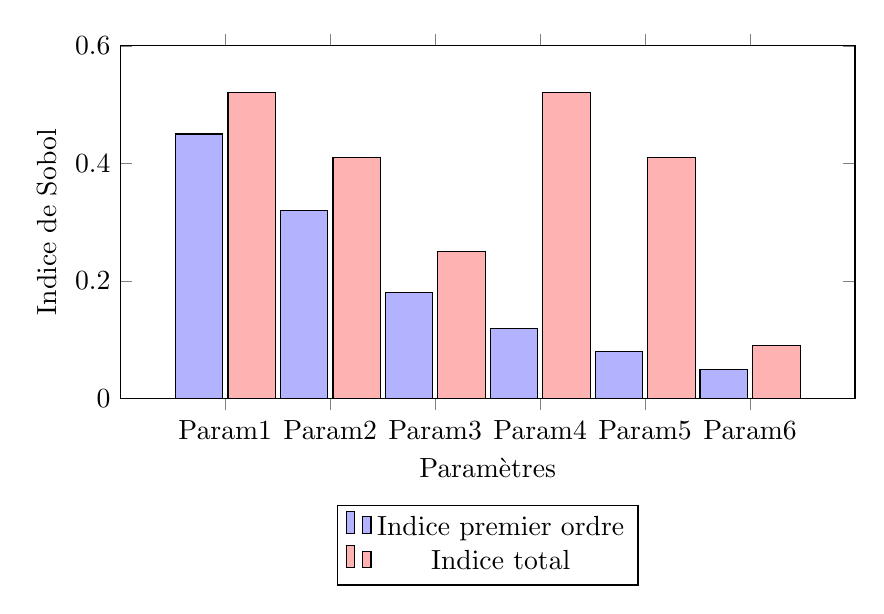
\begin{tikzpicture}
		\begin{axis}[
				width=0.9\textwidth,
				height=0.5\textwidth,
				xlabel={Paramètres},
				ylabel={Indice de Sobol},
				symbolic x coords={Param1, Param2, Param3, Param4, Param5, Param6},
				xtick=data,
				ymin=0,
				ymax=0.6,
				legend style={at={(0.5,-0.3)}, anchor=north},
				ybar,
				bar width=0.6cm,
				enlarge x limits=0.2
		]
			\addplot[fill=blue!30] coordinates{
				(Param1, 0.45) (Param2, 0.32) (Param3, 0.18)
				(Param4, 0.12) (Param5, 0.08) (Param6, 0.05)
			};
			
			\addlegendentry{Indice premier ordre}
			
			\addplot[fill=red!30] coordinates{
				(Param1, 0.52) (Param2, 0.41) (Param3, 0.25)
				(Param4, 0.52) (Param5, 0.41) (Param6, 0.09)
			};
			\addlegendentry{Indice total}
		\end{axis}
	\end{tikzpicture}
	\caption{Analyse de sensibilité par indices de Sobol}
	\label{fig: sensitivity-analysis}
\end{figure}

\section{Équation de performance théorique}

\subsection{Borne de  Cramér-Rao}

la variance d'un estimateur non biaisé est bornée par :

\begin{equation}
	\text{Var}(\hat{\theta}) \geq \frac{1}{I(\theta)}
	\label{eq:cramer-rao}
\end{equation}

Ou $I(\theta)$ est l'information de Fisher.

\subsection{Théorème de limite centrale}

pour des variables i.i.d. avec espérance $\mu$ et variance $\sigma^2$:

\begin{equation}
	\sqrt{n}(\bar{X}_n - \mu) \xrightarrow{d} \mathcal{N} (0, \sigma^2)
	\label{eq:central-limit}
\end{equation}

\subsection{Inégalité de Bernstein}
Pour des variables bornées : 

\begin{equation}
	\mathbb{P}\left(\left|\frac{1}{n}\sum_{i=1}^n X_i - \mu\right| \geq \epsilon\right) \leq 2\exp\left(-\frac{n\epsilon^2}{2\sigma^2 + \frac{2}{3}M\epsilon}\right)
	\label{eq:bernstein-inequality}
\end{equation}